\documentclass[conference,11pt,letterpaper]{IEEEtran}

\usepackage[english]{babel}
\usepackage{csquotes}

\usepackage{fancyhdr}
\usepackage{extramarks}
\usepackage{mathtools}
\usepackage{amsthm}
\usepackage{amsfonts}
\usepackage{tikz}
\usepackage{algorithm}
\usepackage{algorithmicx}
\usepackage{algpseudocode}
\usepackage{setspace}
\usepackage{enumerate}
\usepackage{hyperref}
\usepackage{siunitx}
\usepackage{chngcntr}
\usepackage{graphicx}
\usetikzlibrary{automata,positioning}
\usepackage{wrapfig}
\usepackage{todonotes}
\usepackage{subcaption}
\usepackage{todonotes}
\usepackage{cleveref}
\usepackage{caption}
\usepackage{booktabs}

\captionsetup{font={footnotesize,it},labelfont={footnotesize,bf,it}}

\usepackage[style=authoryear,citestyle=authoryear-comp,maxcitenames=1,backend=biber,backref=false,doi=false,isbn=false,url=false,sorting=nyt]{biblatex}

\addbibresource{quadruped-gait-writeup.bib}

\renewcommand{\bibfont}{\footnotesize}
\setlength\bibitemsep{8pt}


\usepackage[no-math]{fontspec}
\setsansfont{DejaVu Sans}%{Arial}
\setmainfont{Linux Libertine O}%{Times New Roman}
\setmonofont{Inconsolata}%{Consolas}


\captionsetup{compatibility=false}

\emergencystretch=\maxdimen
\hyphenpenalty=10000
\hbadness=10000

\begin{document}
%
% paper title
% Titles are generally capitalized except for words such as a, an, and, as,
% at, but, by, for, in, nor, of, on, or, the, to and up, which are usually
% not capitalized unless they are the first or last word of the title.
% Linebreaks \\ can be used within to get better formatting as desired.
% Do not put math or special symbols in the title.
\title{\LARGE Studying Quadrupedal Gaits in Simulation\\\Large An Optimization-Inspired Approach}

% author names and affiliations
% use a multiple column layout for up to three different
% affiliations
\author{\IEEEauthorblockN{Alexander Volkov}
\IEEEauthorblockA{Robotics Institute\\
Carnegie Mellon University\\
5000 Forbes Ave., Pittsburgh, PA 15213\\
\texttt{avolkovjr@cmu.edu}}}

% make the title area
\maketitle

% As a general rule, do not put math, special symbols or citations
% in the abstract
\begin{abstract}

Of special interest in the study of legged locomotion is the variety of steady-state gaits exhibited by biological quadrupeds, as well as their preference for certain gaits based on locomotive efficiency and desired speed. This work shows that a similar collection of gaits and selection policy naturally emerges for a robotic quadruped. To this end, a high-fidelity dynamic model of the quadrupedal Ghost Robotics \emph{Minitaur} robot was developed and its emergent gait properties studied in simulation.
\end{abstract}

\section{Introduction}

% The introduction should introduce readers to the broader field within which your work is placed, and then guide them to the specific problem that you are addressing and why. Appropriately referencing the work of others to support claims made in the introduction is important here.

The variety of steady-state gaits exhibited by biological quadrupeds has long been of great interest in biomechanics. Previous work \autocite{hoyt_taylor_1981,hegland_taylor_1988} has associated such gait preference in a variety of wild and domestic animals with minimization of power expenditure, depending on desired speed. The ubiquity of this phenomenon in the biological domain motivates an effort to investigate whether a similar gait variety and selection policy naturally emerges on a robotic quadruped, despite the significantly different energy storage, transmission, and actuation mechanisms involved.

In this work, a high-fidelity dynamic model of a quadrupedal robot platform is used to generate and study the emergence of various steady-state gaits commonly observed in biological quadrupedal systems. A na{\"i}ve control architecture consisting of an elliptical foot trajectory generator, softly-tuned joint position PID controllers, and a low-dimensional gait timing parametrization (inspired by \autocite{Hildebrand701}) are used to emphasize the inherent, open-loop robustness of the system for valid gaits. 

Previous efforts on this project yielded promising initial results, but were largely impeded by the difficulty in achieving sufficient sampling granularity over the gait parameter space due to the brute-force evaluation approach taken and the nontrivial time required to compute each simulation trial. 

A more effective sampling method was desired, with the property that it would be biased toward greater sampling granularity near the sparsely distributed regions of interest corresponding to the quadruped's stable gaits. Recognizing that the evaluation of each sample provides an inherent performance metric (the gait efficiency, see \cref{sec:performance}) with local maxima corresponding to the regions of interest, the desired sampling method was reinterpreted as a form of optimization. However, rather than exclusively consider the terminal result of the optimization process, all intermediate steps of the search would be retained to construct a sampled approximation of the gait efficiency over the parameter space. Additional minor considerations would also be required to ensure that such an optimization algorithm is biased against early termination, in favor of searching more aggressively for alternative regions of interest in the parameter space.

The Covariance Matrix Adaptation Evolution Strategy (CMA-ES) optimization algorithm \autocite{hansen2001} was selected based on the foregoing considerations. A brief overview of the algorithm is provided in \cref{sec:cmaes}. A custom \emph{MATLAB} implementation of the CMA-ES algorithm was developed in order to make use of the computing environment's parallelization capabilities as well as interface directly with an existing \emph{Simulink/Simscape Multibody} physics simulation environment from previous work on this project. The resulting pipeline samples the gait parameter space far more efficiently than the previously used brute-force approach.

\subsection{Performance Evaluation} \label{sec:performance}

For the purposes of this study, gait performance was evaluated exclusively in terms of efficiency. Robustness to environmental disturbances was not of concern; a flat, high-friction ground model is used throughout the study. As is standard in locomotion literature \autocite{von1950price}, steady-state gait performance was quantified using the cost of transport (CoT) metric, as per \cref{eq:cot}:

    \begin{equation} \label{eq:cot}
        \text{CoT} = \frac{P_{in_{avg}}}{m_{sys}gv_{avg}} = \frac{E_{in_{tot}}}{m_{sys}gd_{tot}}
    \end{equation}
where $P_{in_{avg}}$ and $E_{in_{tot}}$ are the average power and total energy, respectively, provided to the system over a fixed time period in steady-state locomotion; $v_{avg}$ and $d_{tot}$ are the average velocity of and total distance travelled by, respectively, the system over the same interval; $m_{sys}$ is the total system mass; and $g$ is the acceleration due to gravity.

It should be noted that gait stability and efficiency are highly coupled. Infeasible or otherwise unstable gaits result in very high CoT evaluations, whereas stable gaits are comparably far more energetically effective.

\subsection{CMA-ES Algorithm} \label{sec:cmaes}

	The CMA-ES algorithm was originally reported in \autocite{hansen2001}, building on existing work done in the broader class of algorithms known as \emph{evolutionary strategies} which take inspiration from biological evolution. Generally, such are well suited to nonlinear optimization problems where objective function gradients are not easily computable. CMA-ES, in particular, has gained significant popularity in recent years due to its computational efficiency, making it a popular choice for derivative-free, nonlinear optimization over high-dimensional parameter spaces. 
	
	Conceptually, CMA-ES operates by iteratively modifying a multivariate normal distribution over the parameter space. At each iteration -- a \emph{generation} -- of the algorithm, the distribution is used to sample the parameter space for the following generation, which in turn distorts and moves the distribution in the general direction of greater fitness. The shape of the distribution reflects the focus of the algorithm over the parameter space -- as the algorithm converges upon a local maxima, the distribution will generally tighten. However, in order to avoid premature convergence, a variety of modifications to the algorithm may also be introduced to cause it to broaden its search for alternative regions of high fitness in the parameter space.
	
	
	\begin{algorithm}
		\caption{CMA-ES algorithm}
		\label{alg:cmaes}
		\begin{algorithmic}[1]
			\Function{CMA-ES}{$\lambda \in \mathbb{R},m_0 \in \mathbb{R}^n,\sigma_0 \in \mathbb{R}^{n\times n}$}
			\Statex
			\State $m \gets m_0$  \Comment{Mean}
			\State $\sigma \gets \sigma_0$ \Comment{Std. Dev.}
			\State $C \gets I_{n}$ \Comment{Normalized Covariance}
			\State $p_{\sigma},p_c \gets 0$ \Comment{Evolution Paths}
			\State $gen \gets 1$ \Comment{Generation Counter}
			\State $f \gets 0$ \Comment{Fitness Vector}
			\Statex
			\While{\Call{terminate}{$gen$,$f$} = \texttt{false}}
			\Statex
			\For{$i \gets 1,\lambda$}
			\State $x_i \sim \mathcal{N}(m,\sigma^{2}C)$
			\State $r_i \gets$ \Call{simulate}{$x_i$}
			\State $f_i \gets$ \Call{fitness}{$r_i$}
			\EndFor
			\Statex
			\State $x \gets$ \Call{Sort}{$x,f$} 
			\State $\bar{m} \gets m$ 
			\State $m \gets$ \Call{Mean}{$x$}
			\State $p_\sigma \gets$ \Call{updatePs}{$p_\sigma$,$\sigma$,$C$,$m$,$\bar{m}$}
			\State $p_c \gets$ \Call{updatePc}{}
			\State $C \gets$ \Call{updateC}{}
			\State $\sigma \gets$ \Call{updateSigma}{}
			\State $gen \gets gen+1$
			\Statex
			\EndWhile
			\EndFunction
		\end{algorithmic}
	\end{algorithm}
	
	The basic CMA-ES algorithm is outlined in \cref{alg:cmaes}. The process is initialized by a choice of generational population size $\lambda$, as well as initial mean $m_0$ and standard deviation $\sigma_0$ for the first generation population sampling. Additionally, the normalized covariance matrix $C$ and the two evolutionary path vectors $p_\sigma$ and $p_c$ are instantiated to the identity and null, respectively, as their default values.
	
	During each generation, a population of sampled parameter vectors $x$ is generated from a normal distribution based on the current values of the mean $m$, standard deviation $\sigma$, and normalized covariance matrix $C$. Each parameter vector of the population is then evaluated by the objective function and assigned a fitness value. The population is then sorted by fitness and the parameters of the sampling normal distribution for the next generation are updated. 
	
	The termination conditions for the optimization are checked before each successive generation. For our purposes, the termination conditions were set based on generation count and wall clock time, in order to allow the algorithm to explore the parameter space beyond any given local minima. In most cases, however, the termination will depend primarily on the present and possibly previous generation's fitness values, in order to detect if some form of convergence has occurred.

The CMA-ES code developed for this project was adapted from Nikolaus Hansen's sample \emph{MATLAB} CMA-ES implementation \autocite{Hansen2011}. 


\subsection{Minitaur Robot}

The simulated gait investigation reported here was carried out using a detailed dynamic model of a \emph{Ghost Robotics Minitaur} \autocite{grminitaur}: an 8 DOF, direct-drive (PMSM actuated) quadrupedal robot platform capable of both quasi-static and dynamic gaits. A photo of the \emph{Minitaur} is provided in \cref{fig:grminitaur}. Notably, the legs of this quadruped consist of nearly symmetric five-bar linkages. The robot is approximately 50\si{\centi\m} long, 30 \si{\centi\m} wide, and has a maximal leg extension of 30 \si{\centi\m}. The total weight of the system is 6.36\si{\kg}.

\begin{figure}[ht!]
    \centering
    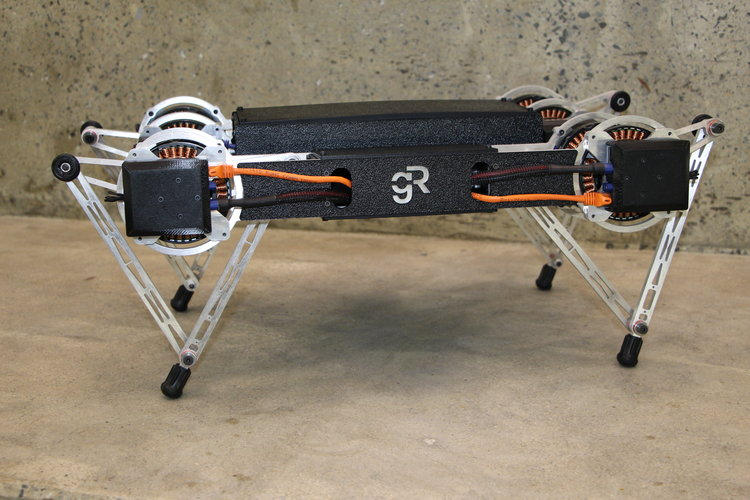
\includegraphics[width=0.48\textwidth]{grminitaur}
    \caption{Ghost Robotics Minitaur \autocite{grminitaur}}
    \label{fig:grminitaur}
\end{figure}

\section{Simulation Model}

Although spring-mass models such as SLIP and LIPM are popular for gait synthesis and control in contemporary legged robotics literature \autocite{albertwuhartmutgeyer2013}, their low-dimensional nature does not capture the complex dynamics that result with respect to both the variety of possible quadrupedal gaits as well as their relationship to the system's locomotive efficiency. Higher-dimensional lumped element models have also been studied as a means of simplifying and abstracting the mechanics of quadrupedal systems while nonetheless capturing their principle dynamic behaviors \autocite{remy2011optimal,full1999templates}. The construction of such reductive models inherently depends on a-priori knowledge of the systems' principle dynamics.

For this investigation, however, a high-fidelity model is needed in order to accurately capture the full system dynamics and power expenditure of the system. In effect, this maximally avoids introducing any simplifications that may inadvertently alter the emergent gait patterns and selection policies.

To this end, a detailed model of the \emph{Minitaur} was previously created in \emph{Simulink/Simscape Multibody} and improved for the work reported here. Descriptions of the various components of the model are given below.

\subsection{Robot Model}
The kinematic, inertial, and graphical properties of the \emph{Minitaur} simulation model were extracted directly from an accurate CAD model supplied by Ghost Robotics. Additional secondary parasitic effects such as joint friction were added based on basic empirical verification. The PMSM actuators are represented using a simplified first-order, linear DC motor model with voltage saturation limits. The motor parameters were taken from the manufacturer's specifications. The foot-ground interaction model was based on a third-party \emph{Simscape} contact modeling package \autocite{contactmodel}. Geometrically, the interaction was represented as a sphere-on-plane contact, matching the actual geometry of the rounded foot and idealized flat ground quite closely. Normal forces were approximated by a linear spring-damper model. A Coulomb stick-slip model was used to model the tangential friction forces. Coefficients were selected to match a realistic scenario of the robot stepping on a carpeted floor.

\subsection{Foot Trajectory Generator and Gait Parametrization}
As noted prior, a very naive approach was taken to the foot trajectory design in order to emphasize the open-loop, steady-state robustness of the resulting gaits. In particular, a prototypical elliptical workspace trajectory was shared by all feet, differing only in phase. The spatial aspects of the trajectory -- the major and minor diameters of the ellipse, its distance from the motor axis, and its tilt relative to the horizon -- were determined manually by examining the reachable workspace of the foot as well as simulation behavior in order to ensure reliable tracking controller performance. \cref{table:traj-params} gives the values used for the spatial parameters of the foot trajectory in this study.

\begin{table}[ht!]
	\centering
	\caption{Foot Trajectory Spatial Parameters}
	\label{table:traj-params}
	\begin{tabular}{@{}ll@{}}
		\toprule
		Parameter                  & Value \\ \midrule
		Ellipse Semi-Major Axis    & 150\hfill[\si{\mm}]   \\
		Ellipse Semi-Minor Axis    & 60\hfill[\si{\mm}]  \\
		Ellipse Tilt               & 0\hfill[\si{\radian}]   \\
		Motor Axis Vertical Offset & 250~\hfill[\si{\mm}]  \\ \bottomrule
	\end{tabular}
\end{table}

Varying the temporal parameters of the trajectory enabled the generation of various gaits. Motivated by biomechanics literature, the quadruped (horse) gait parametrization of \autocite{Hildebrand701} was adapted. In this framework, gaits are divided into two categories -- symmetric and anti-symmetric across the sagittal plane. Note that a number of common gaits, such as the gallop, do not fit into either category, and as such are not considered here. Within both categories, gaits are parametrized by their repetition period and the phase offset between the front and rear legs.

\subsection{Motor Controllers}
Owing to the simple five-bar linkage geometry of the legs, an analytical inverse kinematics model is used to compute desired motor angle from each foot's workspace trajectory. These desired joint angles are then fed into a softly-tuned position PID controller to compute desired motor torques, which are then sent to the motors. The "softness" of the position controller was used to emulate compliance in the leg actuation. The controller gains, common across all four legs, were manually tuned to achieve acceptable performance. 

\section{Results}

The ultimate goal of this endeavor is to find any latent, dimensionless relationships between the morphology of a quadruped and its preferred (low CoT) gaits. To this end, the purpose of this initial work is to demonstrate the evaluation of gait performance for a particular morphology -- namely, the \emph{Minitaur} robot. Using the gait parametrization framework described prior, the parameter space was sampled using CMA-ES and the resulting gaits simulated in order to construct a CoT heatmap over the parameter space.

\subsection{Preliminary Results}
An initial search was carried out over a large range of the parameter space, covering the \emph{period} $t \in (0.5,4) [\si{\s}]$ and the \emph{phase offset} $l \in (0,2\pi) [\si{rad}]$ for both symmetric and anti-symmetric gaits.

The resulting CoT heat map for left/right symmetric gaits is shown in \cref{fig:sync_gait}. A major portion of the evaluated parameter space corresponding to long gait periods resulted in very high CoT values, indicating infeasible gaits. Visualizations of simulated gaits belonging to this region of the parameter space made clear that the long gait periods provided insufficient momentum to move the quadruped forward. However, a number of local minima in CoT (blue) can be seen in the region of shorter gait periods; these correspond to various bounding and pronking gaits, where the quadruped was able to achieve sufficient momentum within each gait cycle to periodically detach its feet from the ground and step forward.
           \begin{figure}[ht!]
   
           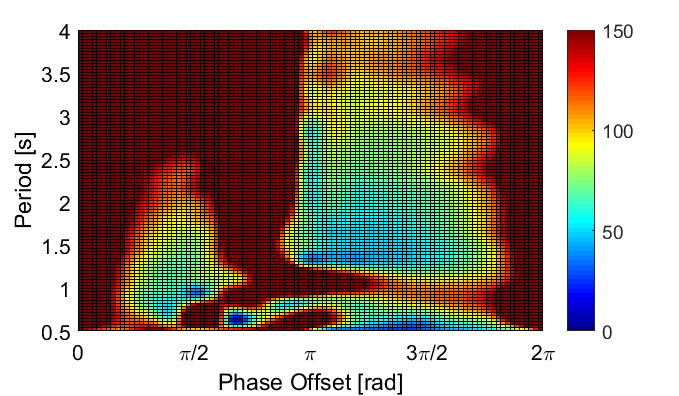
\includegraphics[width=0.53\textwidth]{smooth_CoT_sync_gait}
           \caption{CoT for left/right symmetric gaits}
           \label{fig:sync_gait}
           \end{figure}
                      \begin{figure}[ht!]
The CoT heat map for left/right anti-symmetric gaits similarly yielded local minima which corresponded with walking and trotting gaits (\cref{fig:unsync_gait}). In both heat maps, the minimum CoT occurred at relatively short gait periods, comparable to those seen in similarly sized biological quadrupeds.
           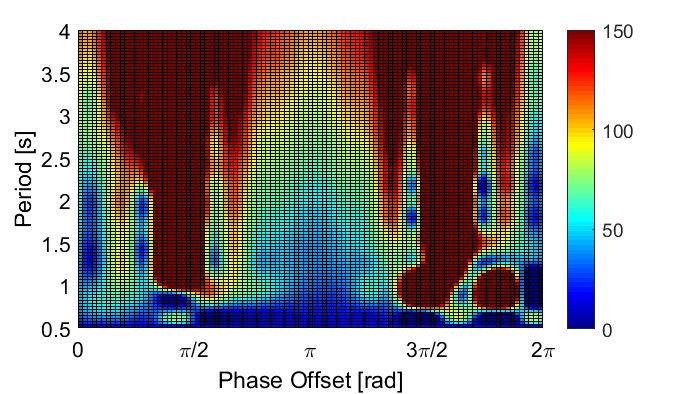
\includegraphics[width=0.53\textwidth]{smooth_CoT_unsync_gait}
           \caption{CoT for left/right anti-symmetric gaits}
           \label{fig:unsync_gait}
           \end{figure}
       
\subsection{Refined Search Space Results}
Since most of the interesting results -- the frequent appearance of CoT minima -- occurred in the parameter space region of short gait periods, the procedure above was repeated over a smaller range of gait periods, between 0.25 [\si{\s}] and 1 [\si{\s}]. The range of evaluated phase offsets remained unchanged.

The minimum CoT found for left/right symmetric gaits was 34.6, occurring at a period of 0.58 [\si{\s}] and a phase offset of 1.1$\pi$ [\si{\radian}] (\cref{fig:sync_gait_2}). Notably, the simulation was unstable in every phase offset condition at periods below 0.5[\si{\s}]. In the left/right anti-symmetric gaits, the minimum CoT was 11.5, occurring at a period of 0.33 [\si{\s}] and a phase offset of 0.9$\pi$ [\si{\radian}] (\cref{fig:unsync_gait_2}). The simulation had unstable gaits at every phase offset below 0.45$\pi$ [\si{\radian}] and above 1.1$\pi$ [\si{\radian}]. 
\begin{figure}[ht!]
         
           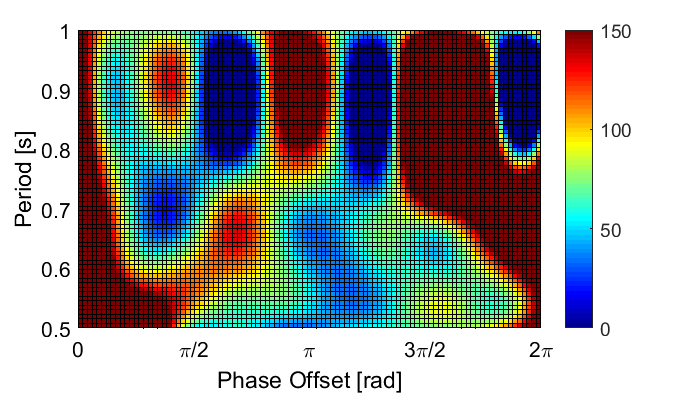
\includegraphics[width=0.53\textwidth]{sync}
           \caption{CoT for left/right symmetric gaits at smaller periods}
           \label{fig:sync_gait_2}
           \end{figure}
           
          \begin{figure}[ht!]
           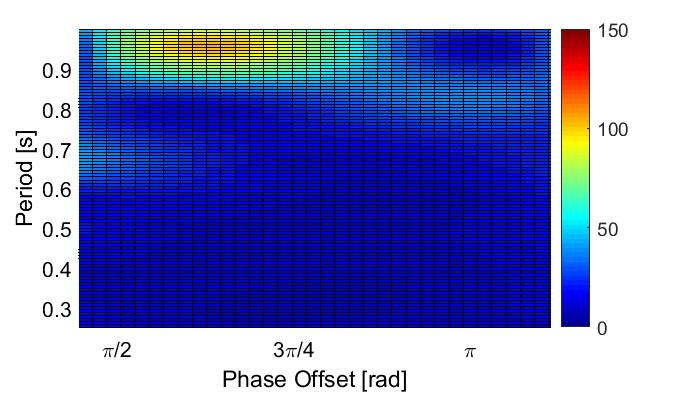
\includegraphics[width=0.53\textwidth]{unsync}
           \caption{CoT for left/right anti-symmetric gaits at smaller periods}
           \label{fig:unsync_gait_2}
\end{figure}
           
\section{Discussion}

Given the same foot trajectories and tracking controllers for all gaits, the most energetically optimal symmetric gait was found at a period of 0.58 [\si{\s}] with a phase offset of 1.1$\pi$ [\si{\radian}]. These parameter values correspond to a bound-like gait. Among the anti-symmetric gaits, the most energetically optimal had a period of 0.33 [\si{\s}] and a 0.9$\pi$ [\si{\radian}] offset, corresponding to a trot. Still frames showing the phases of these gaits are given in \cref{fig:sym_gait,fig:asym_gait}. In Hildebrand's study, horse footfalls were shown throughout a stride in several types of gaits. In running trots, the phase offset between the fore and rear legs was approximately $\pi$, which is similar to the \emph{Minitaur}'s optimal gait of 0.9$\pi$ phase offset \autocite{Hildebrand701}. 

\begin{figure}[t!]
    \centering
    \begin{subfigure}[t]{0.45\linewidth}
        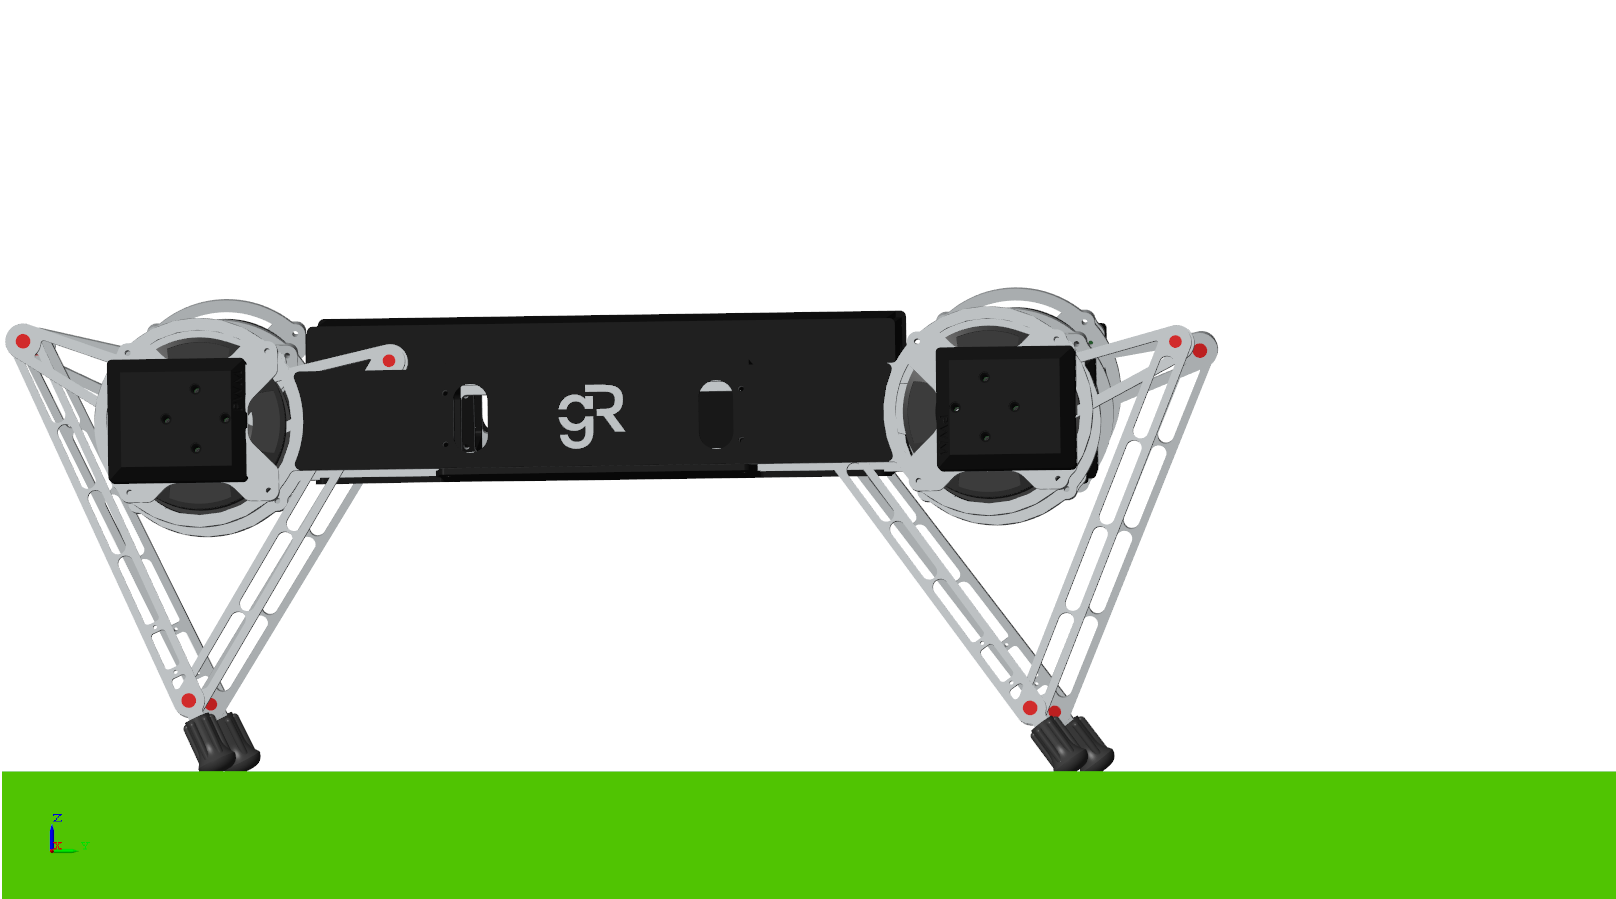
\includegraphics[width=\textwidth]{symm_snap1}
        \caption{State 1}
    \end{subfigure}%
    \begin{subfigure}[t]{0.45\linewidth}
        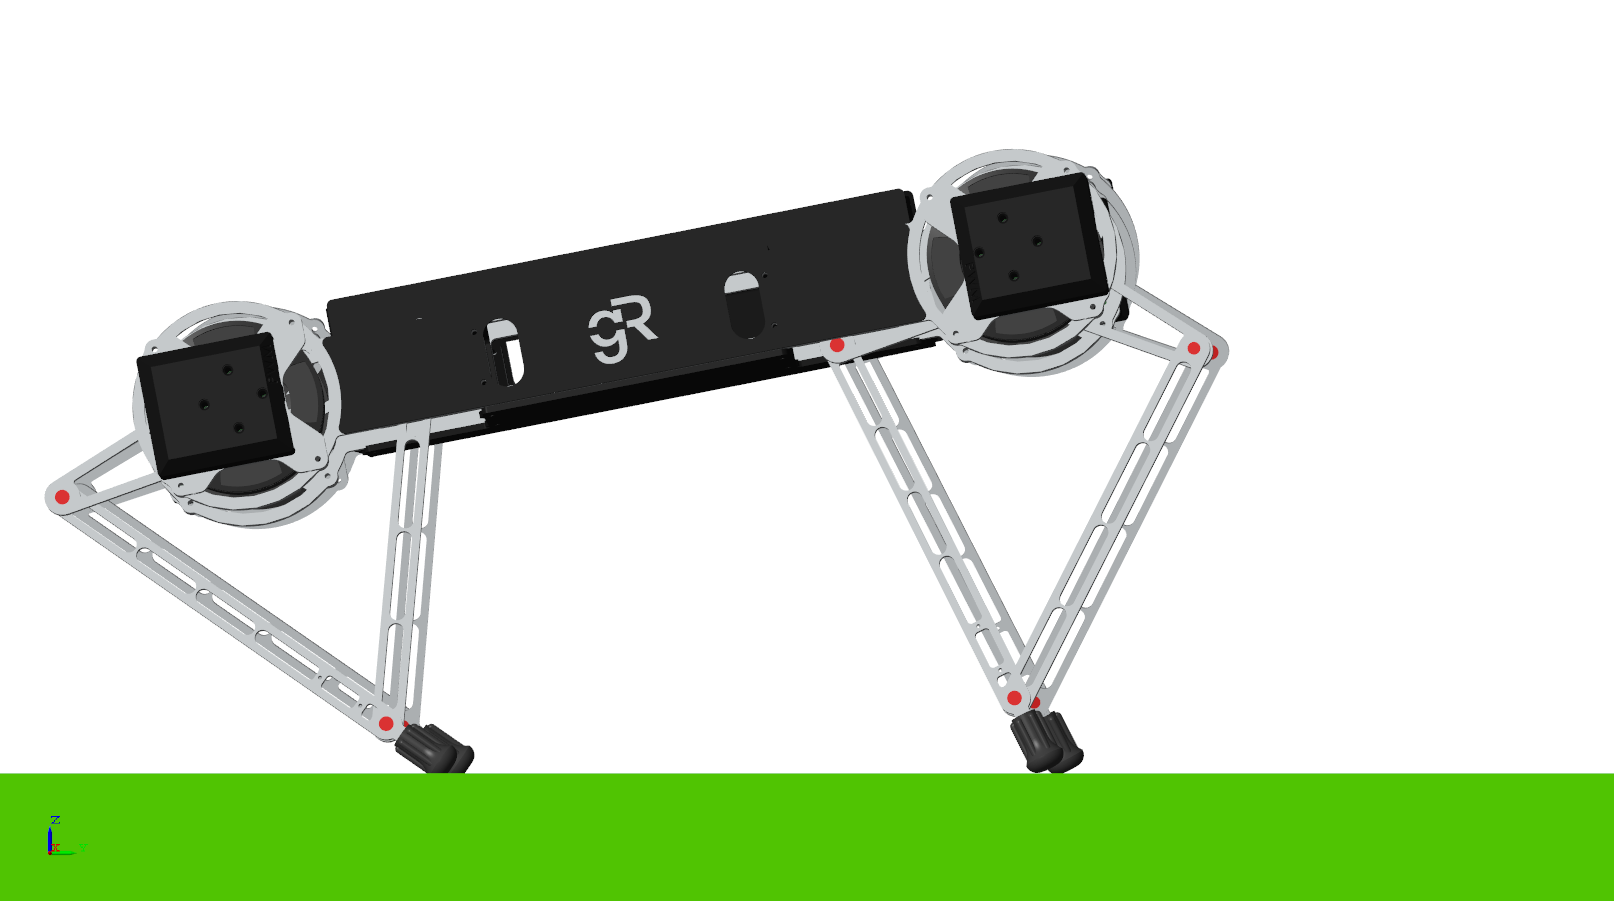
\includegraphics[width=\textwidth]{symm_snap2}
        \caption{State 2}
    \end{subfigure} \\
    \begin{subfigure}[t]{0.45\linewidth}
        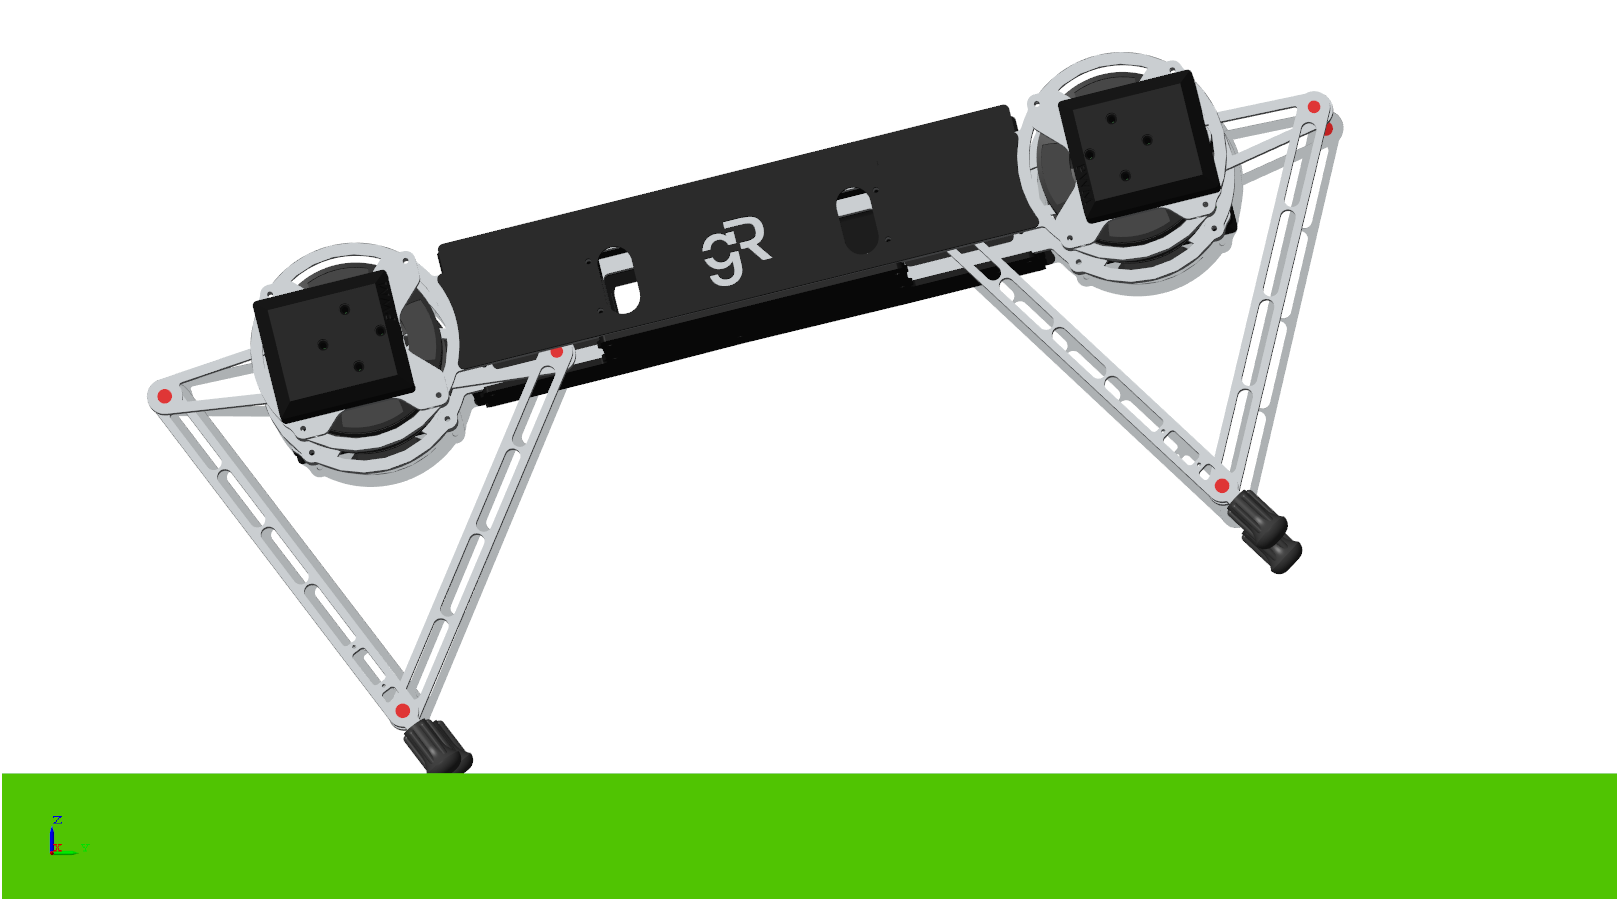
\includegraphics[width=\textwidth]{symm_snap3}
        \caption{State 3}
    \end{subfigure}%
    \begin{subfigure}[t]{0.45\linewidth}
        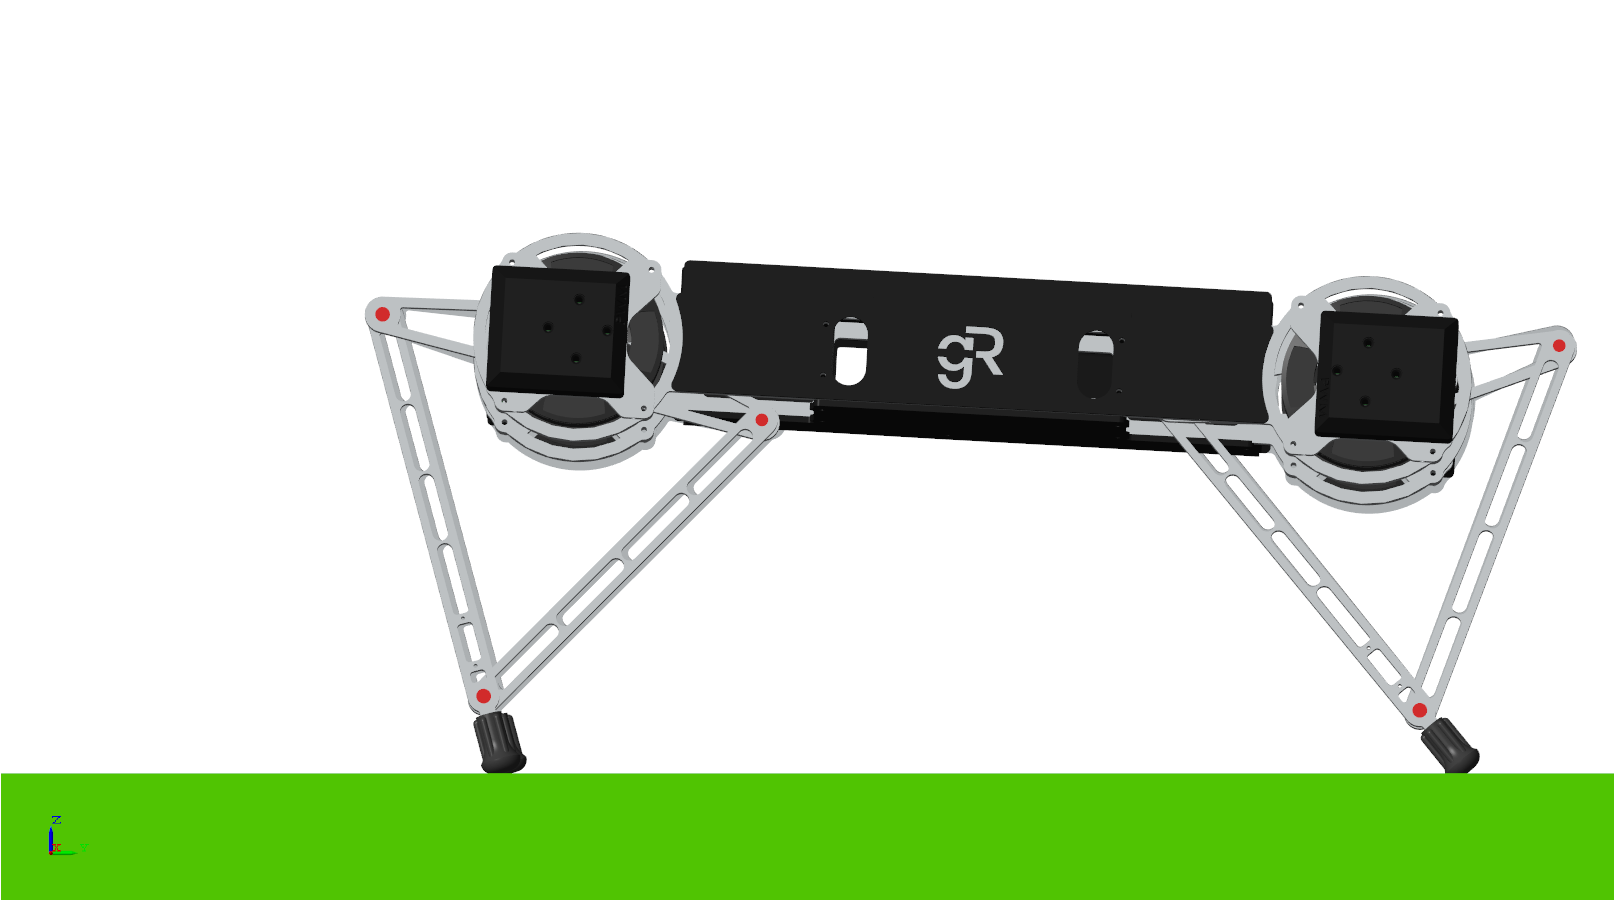
\includegraphics[width=\textwidth]{symm_snap4}
        \caption{State 4}
    \end{subfigure}%
    \caption{Sample symmetric gait with \emph{period} $0.58 s$, \emph{lag} $1.12\pi$}
    \label{fig:sym_gait}
\end{figure}

\begin{figure}[t!]
    \centering
    \begin{subfigure}[t]{0.45\linewidth}
        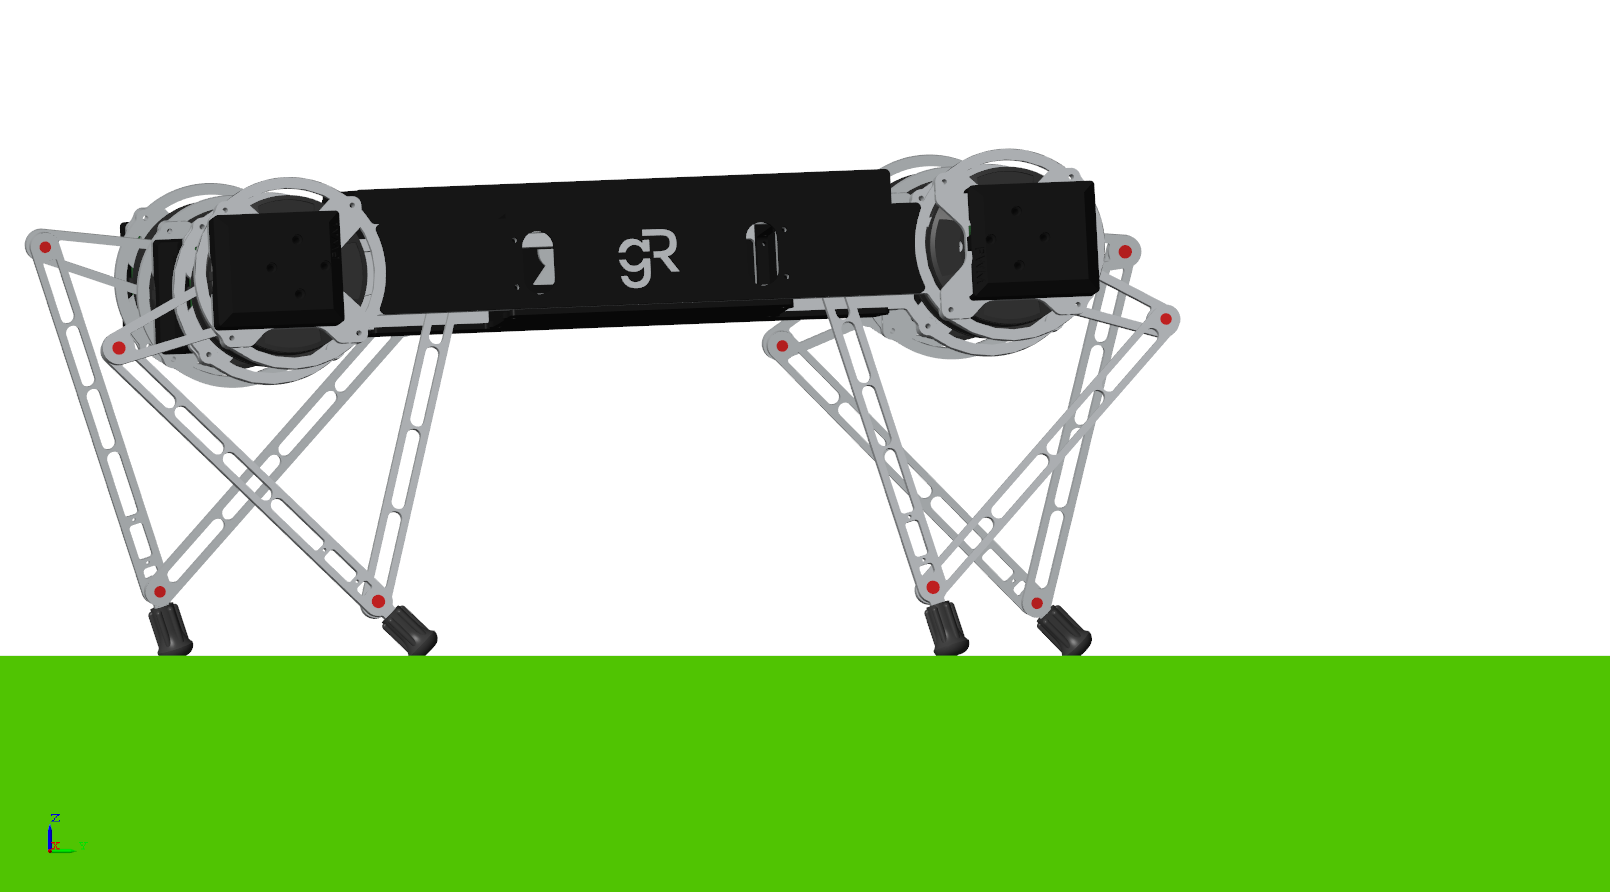
\includegraphics[width=\textwidth]{asymm_snap1}
        \caption{State 1}
    \end{subfigure}%
    \begin{subfigure}[t]{0.45\linewidth}
        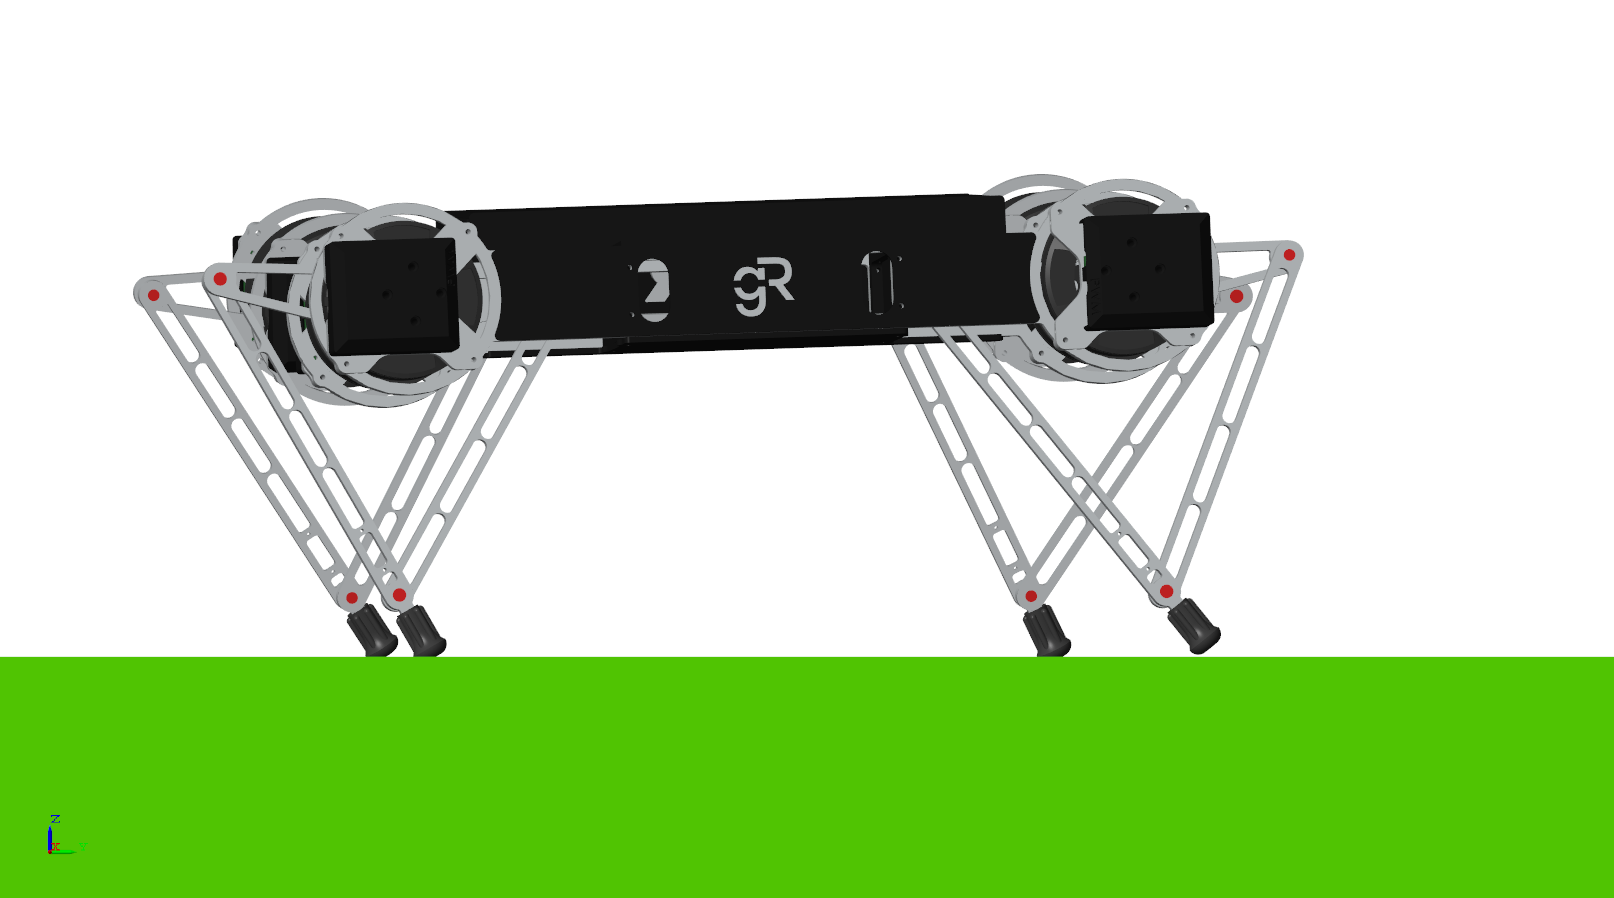
\includegraphics[width=\textwidth]{asymm_snap2}
        \caption{State 2}
    \end{subfigure} \\
    \begin{subfigure}[t]{0.45\linewidth}
        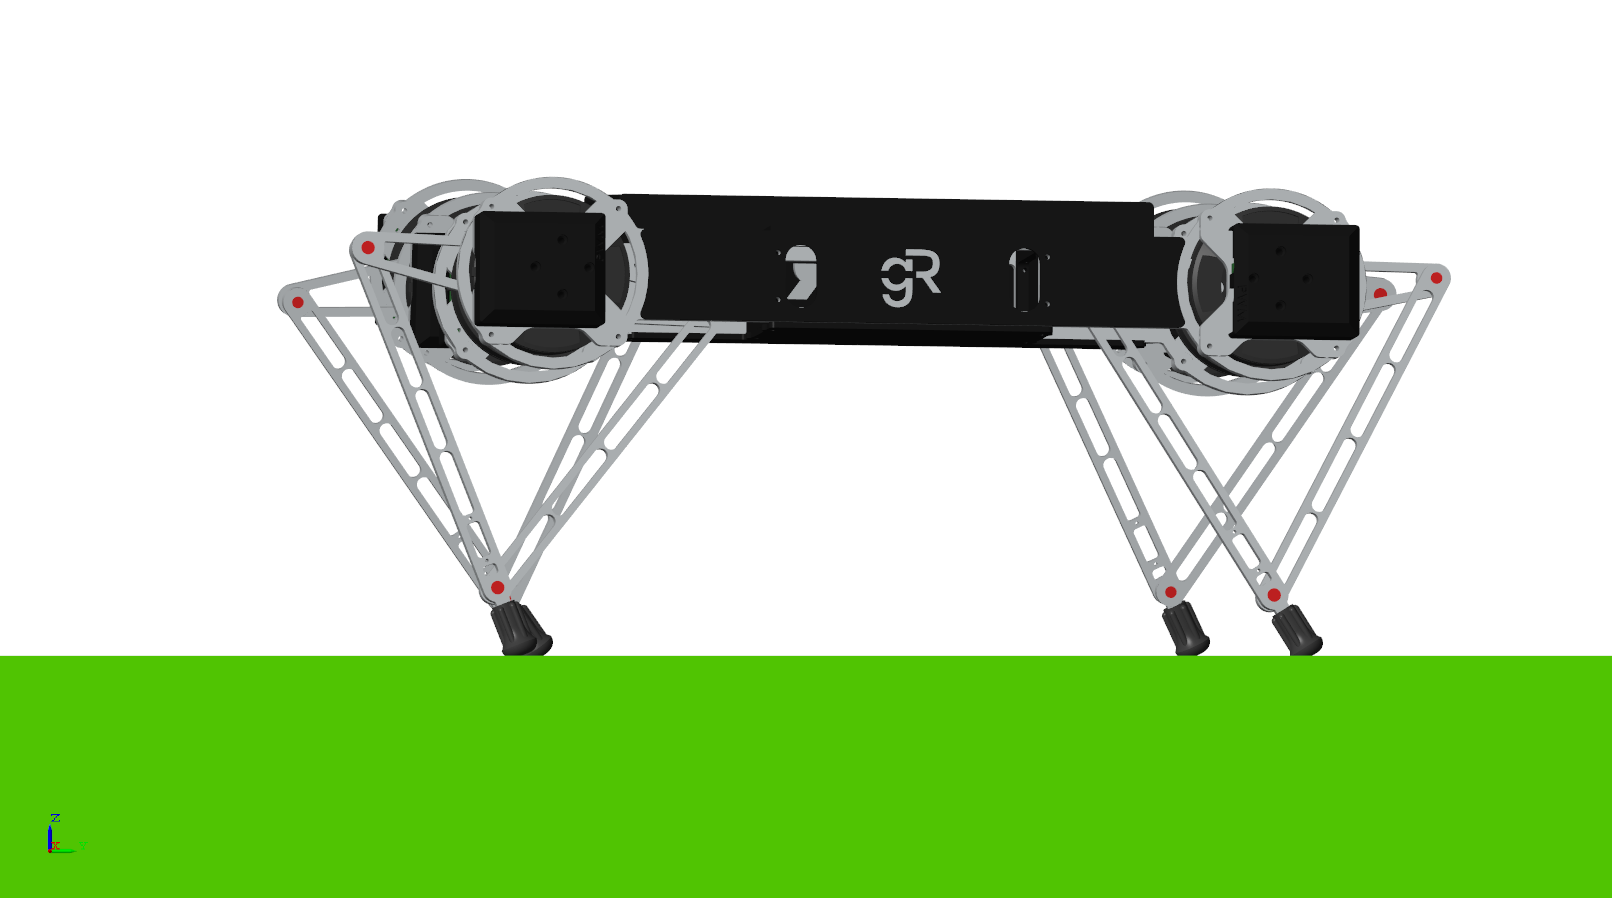
\includegraphics[width=\textwidth]{asymm_snap3}
        \caption{State 3}
    \end{subfigure}%
    \begin{subfigure}[t]{0.45\linewidth}
        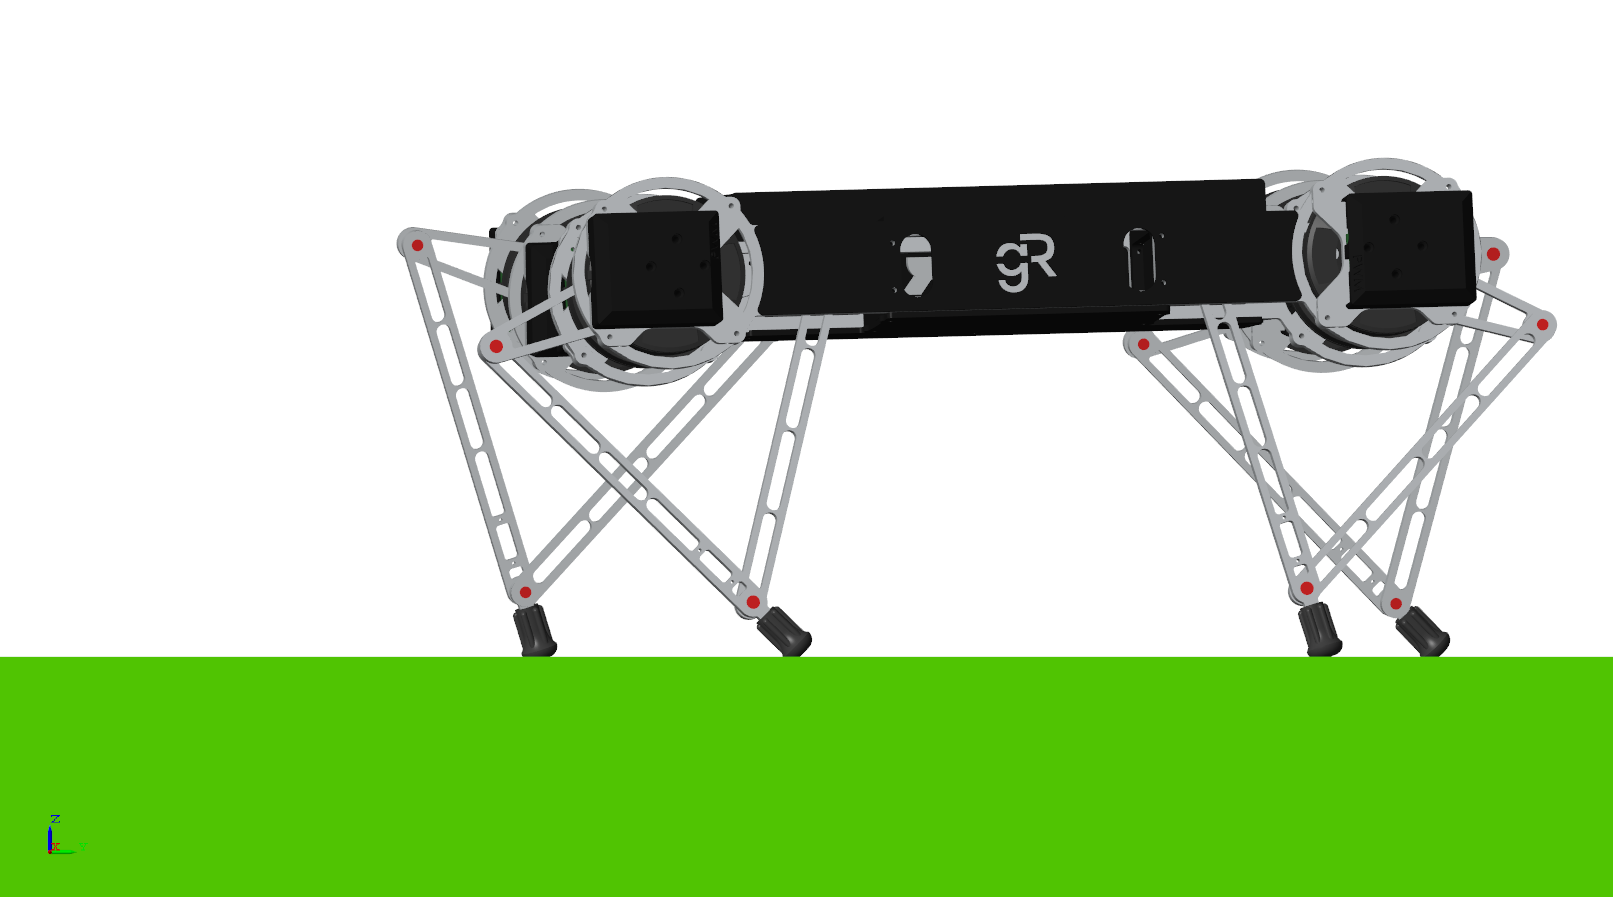
\includegraphics[width=\textwidth]{asymm_snap4}
        \caption{State 4}
    \end{subfigure}%
    \caption{Sample asymmetric gait with \emph{period} $0.33 s$, \emph{lag} $0.9\pi$}
    \label{fig:asym_gait}
\end{figure}

\subsection{Limitations}
The optimal CoT values determined for our models were significantly higher than in biological systems. The minimum CoT discovered by the procedure reported here for the \emph{Minitaur} was 34.6 for left/right symmetric gaits and 11.5 for anti-symmetric gaits while biological systems tend to have CoT values near 0.1-0.15. These high CoT values are not unrealistic for robotic systems, particularly those with direct-drive actuation. However, poor tuning of the foot trajectory tracking controllers could have also contributed to making the gait energetics suboptimal.

The use of CMA-ES for sampling gait parameters proved to be significantly more effective than the brute-force method used previously. However, the optimization approach did yield some additional difficulties in effectively covering the desired space without becoming trapped in local minima. For the results presented here, multiple runs of CMA-ES with different initial conditions were collected and combined as needed.

\subsection{Future Directions}
Ultimately it is desired to use the initial results presented above and the gait generation process as a whole to identify any invariant correlations between quadruped morphology and preferred gaits. This would require an extension to the study in which gait CoT measurements like the ones presented in this work would be repeated for prototypical quadrupeds of varying morphological dimensions. Additionally, future work might also consider evaluation of robustness as an additional metric on gaits. It has been hypothesized that efficient gaits should also have some qualities of robustness, perhaps with regard to imperfections in terrain. The infrastructure developed for this work could be adapted to investigate gait robustness as well.

% use section* for acknowledgment
\section*{Acknowledgment}

The author would like to thank Professor Chris Atkeson for overseeing this independent study, as well as Thu Nguyen (formerly a graduate student at CMU, presently at Stanford) for her previous contributions to the project. Additionally, the author would also like to acknowledge Ghost Robotics LLC for supporting this work by providing design files of the \emph{Minitaur} robot platform. 

\appendix
\section{Project Repository}
In the spirit of open-access distribution of scientific results, all files associated with this project have been made freely available at the following git repository: \url{https://github.com/rustechs/16-995-indep-study/}

% references section
\nocite{*}
\printbibliography

% that's all folks
\end{document}


